\section{Implementation of Solutions}

Colour detection, SURF and chessboard detection were all implemented to evaluate their performance for tracking a marker in the required environment. To aid in this implementation extensive use was made of the Opencv computer vision libraries \cite{opencv}. These libraries were used as they contained implementations of a large number of computer vision algorithms that had been thoroughly tested by a large community and optimized to run as effectively and efficiently as possible.

The first algorithm implemented was the simple colour based approach. In this approach a bright blue ball was used as the marker to track. Initially the scene was thresholded for a value that was approximately  a bright blue and opening (that is erosion followed by dilation) was used to fill any holes in the image of the ball and remove background noise. The output of this process can be seen in Figure~\ref{ball}. A rough estimation of the balls location was then made using its x and y position in pixels from the centre of the camera. The z location of the ball was taken to be proportional to the inverse of the square root of the size of the ball in pixels. These measures of x, y and z were extremely crude however they provided adequate for the testing that was performed on the colour method.

\begin{figure}[ht]
	\begin{center}
		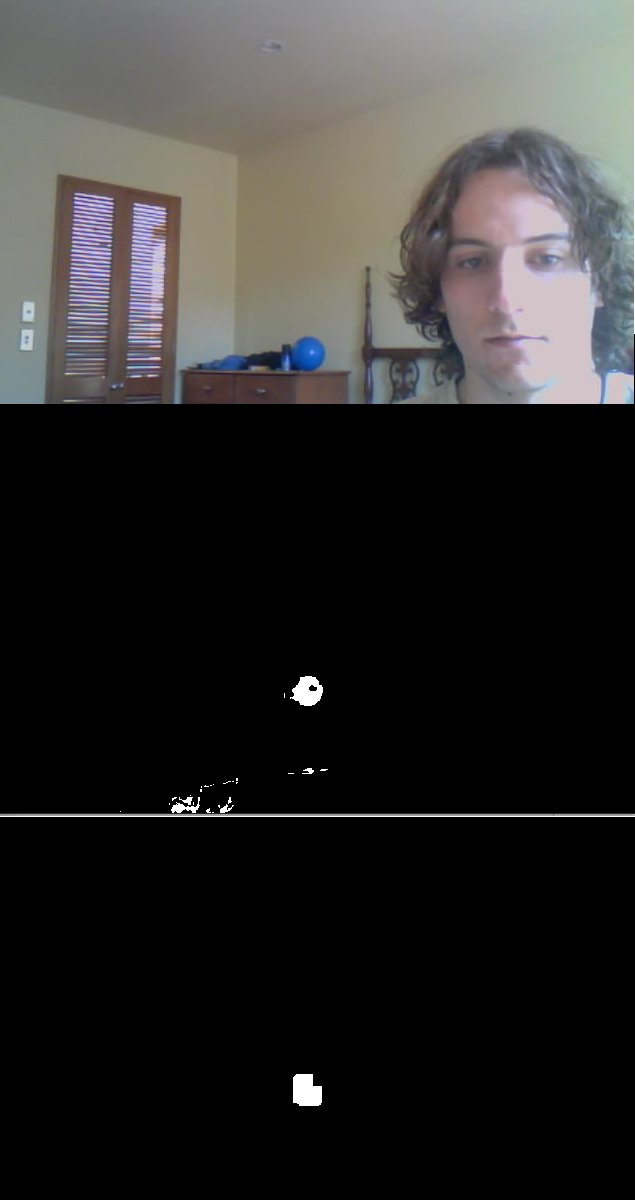
\includegraphics[width=0.3\textwidth]{2}
	\end{center}
	\caption{Detection of marker ball using colour}
	\label{ball}
\end{figure}

For both the SURF and chessboard algorithms the intrinsic parameters of the camera had to be found so that the size of an object on the screen could be translated from the arbitrary pixel co-ordinate system used by the images to real world distances. These parameters were found by using the camera to take a series of photos of the chessboard from different angles and distances and using the geometry of the chessboard to extract the cameras parameters \cite{cali}. Once this had been performed the parameters were saved to a file that was used by both algorithms. This calibration was a small disadvantage of these algorithms however as it only had to be performed once for a web-cam it did not diminish the practicality of their use by much.

The SURF algorithms marker was a printout of a cut away of an aeroplane. This image was used as it contained a large amount of strong lines and detail that meant that a large number of unique and easily identifiable points could be located on the image. An example of the SURF algorithm working can be seen in Figure~\ref{plane}. 

Two chessboards were constructed and tested with the chessboard registration algorithm. A large 6 by 5 chessboard with 100 mm squares and a smaller 7 by 8 chessboard. The larger chessboard was to be used with the kart once it was running. The smaller one was used for calibrating the camera and the testing covered in this report. The smaller board can be seen being used in Figure~\ref{tracking}. 

\begin{figure}[ht]
	\begin{center}
		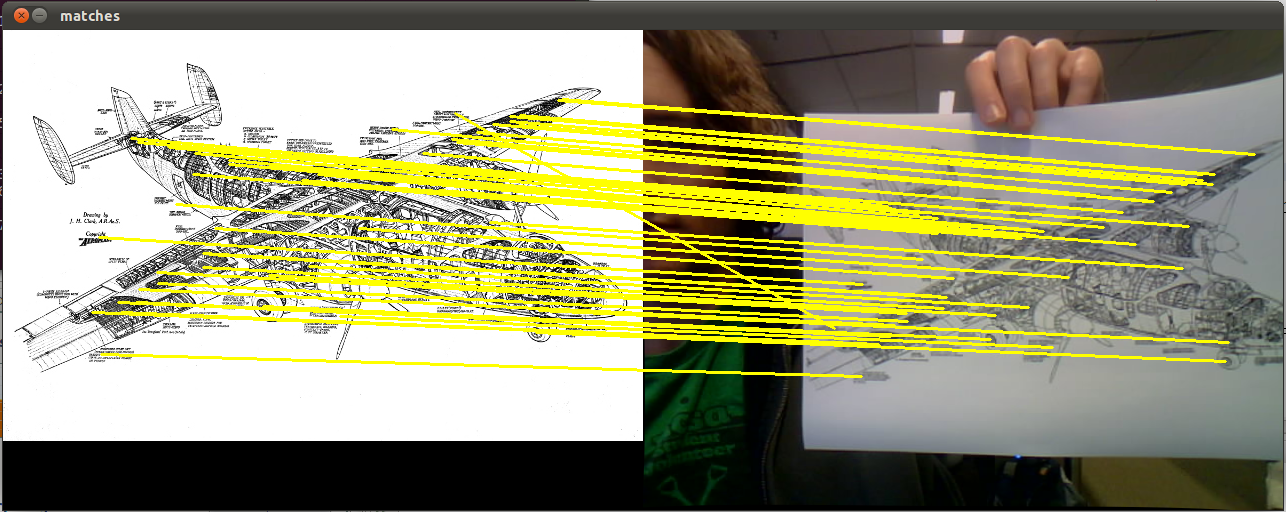
\includegraphics[width=0.5\textwidth]{surf_match}
	\end{center}
	\caption{The SURF algorithm matching points in the marker image to the scene}
	\label{plane}
\end{figure}